
\ifdefined\ishandout
\documentclass[11pt,english,handout]{beamer}
\else
\documentclass[11pt,english]{beamer}
\fi


\usepackage{mathptmx}
\renewcommand{\sfdefault}{lmss}
\renewcommand{\familydefault}{\sfdefault}
\usepackage[T1]{fontenc}
\usepackage[latin9]{inputenc}
\usepackage{amsmath}
\usepackage{amssymb}
\usepackage{graphicx}
\PassOptionsToPackage{normalem}{ulem}
\usepackage{ulem}
\usepackage{caption}
\captionsetup{labelformat=empty}
\usepackage{bbm}
\usepackage{upgreek}
\usepackage{graphicx}
\setbeamertemplate{section in toc}[sections numbered]
\makeatletter
\usepackage{caption} 
\usepackage{bm}
\usepackage{subfig}
\captionsetup[table]{skip=10pt}
\usepackage{pdflscape}
%%%%%%%%%%%%%%%%%%%%%%%%%%%%%% Textclass specific LaTeX commands.
% this default might be overridden by plain title style
\newcommand\makebeamertitle{\frame{\maketitle}}%
% (ERT) argument for the TOC
\AtBeginDocument{%
	\let\origtableofcontents=\tableofcontents
	\def\tableofcontents{\@ifnextchar[{\origtableofcontents}{\gobbletableofcontents}}
	\def\gobbletableofcontents#1{\origtableofcontents}
}

%%%%%%%%%%%%%%%%%%%%%%%%%%%%%% User specified LaTeX commands.
%\documentclass[presentation]{beamer}


\def\Tiny{\fontsize{7pt}{8pt}\selectfont}
\def\Normal{\fontsize{8pt}{10pt}\selectfont}

\usetheme{Madrid}
\usecolortheme{lily}
%\setbeamercovered{transparent}
\useinnertheme{rounded}


\setbeamertemplate{footline}{\hfill\Normal{\insertframenumber/\inserttotalframenumber}}
%\setbeamertemplate{footline}{}

\setbeamertemplate{navigation symbols}{}

\newenvironment{changemargin}[2]{%
	\begin{list}{}{%
			\setlength{\topsep}{0pt}%
			\setlength{\leftmargin}{#1}%
			\setlength{\rightmargin}{#2}%
			\setlength{\listparindent}{\parindent}%
			\setlength{\itemindent}{\parindent}%
			\setlength{\parsep}{\parskip}% 
		}%
		\item[]}{\end{list}}

\setbeamertemplate{footline}{\hfill\insertframenumber/\inserttotalframenumber}
\setbeamertemplate{navigation symbols}{}

%\usepackage{times}  % fonts are up to you
\usepackage{graphicx}
%\usepackage{graphics}
\usepackage{epsfig}
\usepackage{bm}
\usepackage{epsf}
\usepackage{float}
\usepackage[final]{pdfpages}
\usepackage{multirow}
\usepackage{colortbl}
\usepackage{xkeyval}
%\usepackage{sgame}
%\usepackage{pst-node}
\usepackage{listings}
\usepackage{ifthen}
%\usepackage{hyperref}
\usepackage{tikz}

%\usepackage{times}  % fonts are up to you
%\usepackage{graphicx}
%\usepackage{graphics}
\usepackage{epsfig,bm,epsf,float}
\usepackage[final]{pdfpages}
\usepackage{xcolor,multirow,colortbl}
\usepackage{xkeyval}
\usepackage{verbatim}
%\usepackage{sgame}
%\usepackage{pst-node}
\usepackage{listings}
%\usepackage{handoutWithNotes}
%\pgfpagesuselayout{3 on 1 with notes}[letterpaper,border shrink=5mm]
%\pgfpagesuselayout{2 on 1 with notes landscape}[letterpaper,border shrink=5mm]
\usepackage{setspace}
\usepackage{ragged2e}
\usepackage{pdfpages}
\setbeamersize{text margin left=1em,text margin right=1em} % CambridgeUS spacing if you use default instead


%\pdfmapfile{+sansmathaccent.map}

% Table formatting
\usepackage{booktabs}


% Decimal align
\usepackage{dcolumn}
\newcolumntype{d}[0]{D{.}{.}{5}}


\global\long\def\expec#1{\mathbb{E}\left[#1\right]}
\global\long\def\var#1{\mathrm{Var}\left[#1\right]}
\global\long\def\cov#1{\mathrm{Cov}\left[#1\right]}
\global\long\def\prob#1{\mathrm{Prob}\left[#1\right]}
\global\long\def\one{\mathbf{1}}
\global\long\def\diag{\operatorname{diag}}
\global\long\def\expe#1#2{\mathbb{E}_{#1}\left[#2\right]}
\DeclareMathOperator*{\plim}{\text{plim}}

%\usefonttheme[onlymath]{serif}

\usepackage{appendixnumberbeamer}
\renewcommand{\thefootnote}{}

\setbeamertemplate{footline}
{
	\leavevmode%
	%   \hbox{%
	%      \begin{beamercolorbox}[wd=\paperwidth,ht=2.25ex,dp=1ex,right]{date in head/foot}%
	%\usebeamerfont{date in head/foot}\insertshortdate{}\hspace*{2em}%
	\hfill
	%turning the next line into a comment, erases the frame numbers
	\insertframenumber{}\hspace*{2ex}\vspace{1ex}
	
	%    \end{beamercolorbox}}%
}

\definecolor{blue}{RGB}{0, 0, 210}
\definecolor{red}{RGB}{170, 0, 0}

\makeatother

\usepackage[english]{babel}

\usepackage{tikz}
\newcommand*\circled[1]{\tikz[baseline=(char.base)]{             \node[circle,ball color=structure.fg, shade,   color=white,inner sep=1.2pt] (char) {\tiny #1};}} 

\makeatletter
\let\save@measuring@true\measuring@true
\def\measuring@true{%
	\save@measuring@true
	\def\beamer@sortzero##1{\beamer@ifnextcharospec{\beamer@sortzeroread{##1}}{}}%
	\def\beamer@sortzeroread##1<##2>{}%
	\def\beamer@finalnospec{}%
}
\makeatother



\setbeamersize{text margin left= .8em,text margin right=1em} 
\newenvironment{wideitemize}{\itemize\addtolength{\itemsep}{10pt}}{\enditemize}
\newenvironment{wideitemizeshort}{\itemize}{\enditemize}

\newcommand{\indep}{\perp\!\!\!\!\perp} 


\DeclareMathOperator*{\argmax}{arg\,max}
\DeclareMathOperator*{\argmin}{arg\,min}

\begin{document}
	
	%% Title slide
	\begin{frame}[noframenumbering]{}
		\vspace{0.5cm}
		\title[]{Review Session}
		\author{Jonathan Roth}
		\date{Mathematical Econometrics I \\ Brown University\\} 
		\titlepage {\small{}\ }\thispagestyle{empty} \vspace{-30pt}
		
	\end{frame}


\begin{frame}{Overview}
	\begin{enumerate}
		\item 
		Structure of final and logistics
		
		\item
		Key course concepts
		
		\item
		Your questions
	\end{enumerate}
\end{frame}
	
	
\begin{frame}{Structure of final}
	\begin{wideitemize}
		\item
		The structure of the final will be similar to the final from last year
		
		\item
		There will be 1-2 analytical questions that will ask you to use mathematical tools we've learned in this course
		
		\item
		There will be questions about a new empirical application. You will be required to state and evaluate assumptions under which we can learn about causal effects, and comment on empirical results.
		
	\end{wideitemize}
\end{frame}	


\begin{frame}{Logistics for final}
	\begin{wideitemize}
		
		\item
		The final exam will be in-person and 2 hours long
			\begin{wideitemize}
				\item
				Please email me and your TAs if you have a SAS accommodation for extra time
				
			\end{wideitemize}
		
		\item
		The final exam will be December 15 at 2pm in MacMillan Hall 117
		
		\item
		You may bring 2 8.5x11'' pieces of paper with notes
			\begin{itemize}
				\item 
				E.g. your ``cheatsheet'' for the midterm plus a new one
			\end{itemize}
		
	\end{wideitemize}
\end{frame}

\begin{frame}{Overview of course}
	\begin{wideitemize}
		\item
		In this class, we focused primarily on how we can answer \underline{causal} economic questions with data
			\begin{wideitemize}
				\item
				What is the effect of going to Brown versus URI on earnings? 
				
				\item
				What is the effect of gaining health insurance on depression? 
				
				\item
				What is the effect of the minimum wage on employment?
			\end{wideitemize}
		
		\pause
		\item
		We formalized the idea of a causal effect with \textit{potential outcomes}
			\begin{wideitemize}
				\item 
				Each unit has a potential outcome under both treatment and control, $Y_i(1)$ and $Y_i(0)$
				
				\item
				E.g. $Y_i(1) =$ earnings if go to Brown; $Y_i(0)=$ earnings if go to URI
				
				\item
				We observe only $Y_i(1)$ for treated units and $Y_i(0)$ for control units
				
				\item
				We are interested in the causal effect $Y_i(1) - Y_i(0)$ (or averages of this over the population) 
			\end{wideitemize}
	\end{wideitemize}
\end{frame}

\begin{frame}{Two key challenges}

There are two key challenges in answering causal questions with data:	\medskip 
	
	\begin{wideitemize}
		\item
		We never observe the counterfactual outcome for each unit
			\begin{itemize}
				\item
				E.g., we observe earnings for Brown students ($Y_i(1)$), but not their earnings if they'd gone to URI ($Y_i(0)$) 
			\end{itemize} 
		
		\item
		We typically only observe data for a sample rather than for the full population that we care about
		\begin{itemize}
			\item
			E.g., we only have data from a survey of a small fraction of recent graduates 
		\end{itemize}
	\end{wideitemize}

\end{frame}

\begin{frame}{Identification versus Statistical Inference}

We typically tackle these two problems separately: \medskip	
	
	\pause 
	
	\begin{wideitemize}
		\item
		\textbf{Identification:} what could we learn about the causal effect if we had the observable data from the full population? 
		\pause
			\begin{wideitemize}
				\item
				Typically start with some assumptions about how treatment is assigned
				
				\item
				Under these assumptions, show that this causal effect is a function of observable population means
			\end{wideitemize}
		\pause
		\item
		\textbf{Statistical Inference:} what can we learn about the observable features of the population given the sample? \pause
			\begin{wideitemize}
				\item
				Typically estimate population means by plugging in sample means
				
				\item
				When we need to estimate conditional means, we use regression to approximation the CEF
				
				\item
				We can use statistical tools to test hypotheses and construct confidence intervals
			\end{wideitemize}		
	\end{wideitemize}
\end{frame}

\begin{frame}{5 Different Types of Identification Arguments}
	\begin{wideitemize}
		\item
		\textbf{Experiments:} if treatment is randomized, can compare outcomes for treated pop to control pop
		
		\pause
		\item
		\textbf{Conditional unconfoundedness:} assume treatment assignment is like an experiment conditional on observable characteristics --- compare treated/control populations with the same covariates
		
		\pause
		\item
		\textbf{Difference-in-differences:} allow for there to be selection into treatment, but assume selection bias is constant over time --- compare differences after treatment occurs to differences before treatment
		
		\pause
		\item
		\textbf{Instrumental variables:} assume that assignment of an instrument is random and affects outcome only through treatment --- compare populations with different values of the instrument
		
		\pause
		\item
		\textbf{Regression discontinuity:} assume that confounding factors evolve continuously around the cutoff --- compare population with scores just below the cutoff to just above
	\end{wideitemize}	
\end{frame}

\begin{frame}{Experiments}

Sample means of depression
\begin{tabular}{lll}
	& Control Group & Treated Group \\
	Mean & 0.329 & 0.306\\
	SD & 0.470 &  0.461 \\
	N & 10426 & 13315  
\end{tabular}


\begin{wideitemize}
	\item
	Identification: \pause{}$D_i \indep (Y_i(1),Y_i(0))  \implies ATE = E[Y_i | D_i =1 ] - E[Y_i | D_i = 0]$ \\ \medskip Make sure you know how to derive this!
	
	\pause
	\item
	Estimation: replace population means with sample means!
	
	\pause
	\item
	Estimation 2: can also estimate with OLS
	$$Y_i = \alpha + \beta D_i + \epsilon_i$$
\end{wideitemize}
	
\end{frame}


\begin{frame}{Conditional unconfoundedness}
	\begin{wideitemize}
		\item
		Example: maybe where you go to college is as-good-as-random conditional on where you get in (Dale \& Krueger)
		
		\pause
		\item
		Identification: $D_i \indep (Y_i(1),Y_i(0)) | X_i  \implies CATE(x) = E[Y_i | D_i =1 , X_i = x] - E[Y_i | D_i = 0, X_i = x]$ 
		
		\pause
		\item
		Estimation: typically, we need to approximate the CEF $\rightarrow$ use OLS!
		
		\item
		Common to approximate ATE with OLS estimates of 
		
		$$Y_i = \alpha + \beta D_i + \bm{\gamma}' \bm{X_i} + \epsilon_i$$
		
		\pause
		\item
		This works well if (i) conditional unconfoundedness holds, and (ii) the CEF is approximately linear: $E[Y_i | D_i, \bm{X}_i] \approx \alpha + \beta D_i + \bm{\gamma}' \bm{X_i} $
	\end{wideitemize}	
\end{frame}

\begin{frame}
	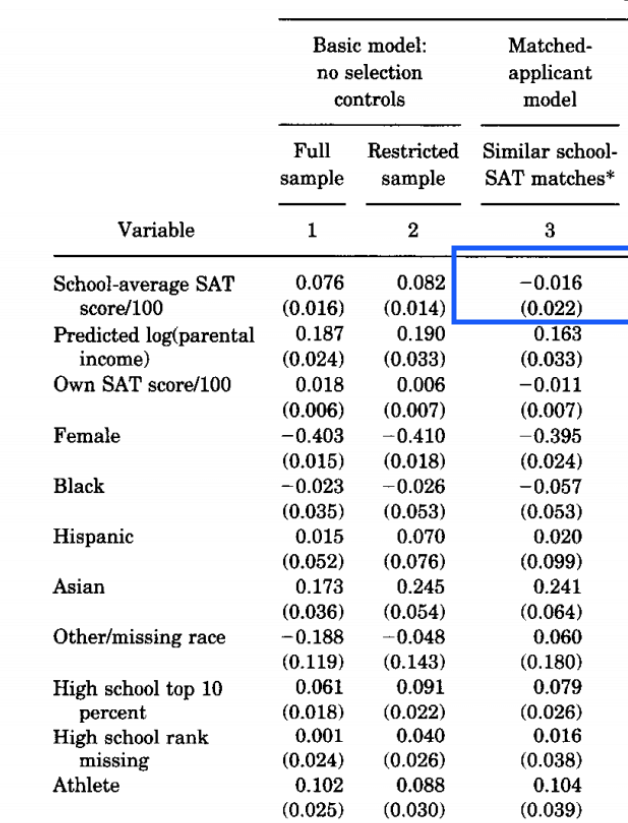
\includegraphics[width = 0.4\linewidth]{dk-results-table-reg2}
\end{frame}

\begin{frame}{Difference-in-differences I}
	\centering
	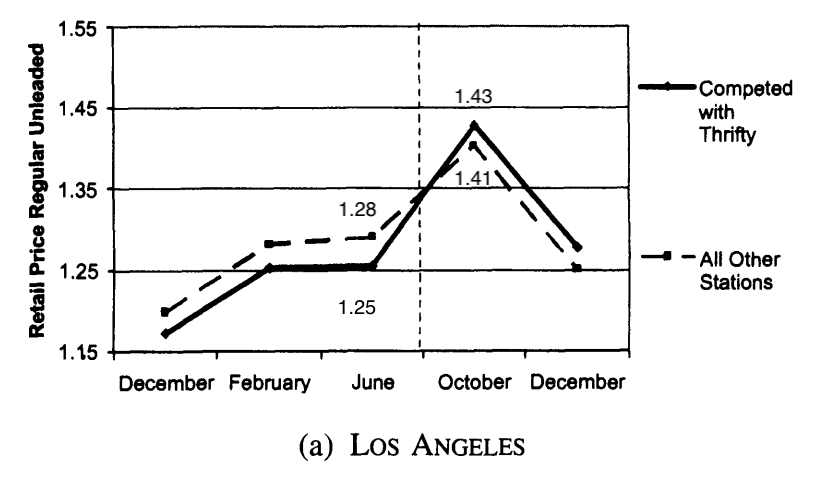
\includegraphics[width = 0.5\linewidth]{../Chapter6/hastings-event-study-w-labels}
	
	\begin{wideitemize}
		\item
		Key identification assumption: parallel trends --- selection bias is constant over time (make sure you know the formal definition)
		
		\pause
		\item
		Identification: under parallel trends (and no anticipation), $\tau_{ATT} = \underbrace{(\mu_{12} - \mu_{11})}_{\text{Change for treated pop}} - \underbrace{ (\mu_{02} - \mu_{01}) }_{\text{Change for control pop}}$
	
		\pause	
		\item
		Estimation: plug in sample means instead of population means!
		
		\pause
		\item
		Estimation 2: can also estimate with OLS (make sure you know how to do this!)
	\end{wideitemize}
\end{frame}

\begin{frame}{Difference-in-differences II }
	\begin{wideitemize}
		\item
		It is common to assess plausibility of DiD assumption by looking at pre-treatment trends with an ``event-study''
		
		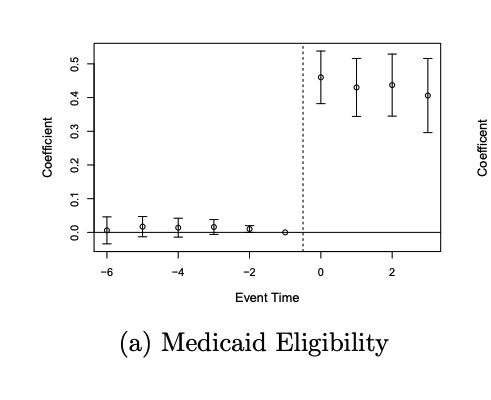
\includegraphics[width = 0.5\linewidth]{../Chapter6/medicaid-eligibility}
		
		\item
		We gain confidence in the research design if (i) pre-trends close to 0, and (ii) can't draw a straight line through all the CIs (there is a break from trend!)
		
		\pause
		\item
		Estimation of the event-study can be done via OLS (make sure you know how!)
	\end{wideitemize}
\end{frame}

\begin{frame}{IV}
	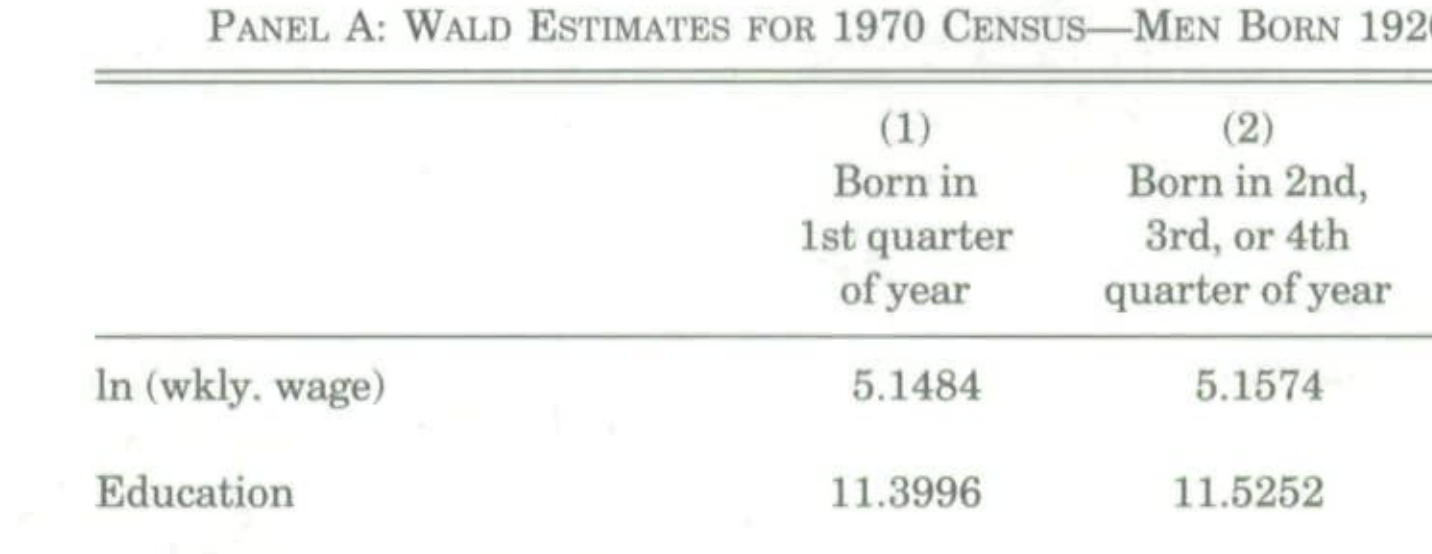
\includegraphics[width = 0.5\linewidth]{../Chapter7/ak-first-stage-basic}
	
	\begin{wideitemize}
		\item
		In IV, we have an instrument that is as-good-as-randomly assigned and affects the outcome only through its effect on the treatment
		
		\item
		Four key identifying assumptions (make sure you understand them!):
		\begin{wideitemize}
			\item
			Independence: instrument is as good as randomly assigned	
			
			\item
			Exclusion: instrument affects outcome only through treatment
			
			\item
			Monotonicity: no defiers
			
			\item
			Relevance: instrument affects treatment status
		\end{wideitemize}	
		 
		
		\pause
		\item
		Under the four key assumptions, $\beta_{IV} = \frac{ E[Y_i | Z_i = 1] - E[Y_i | Z_i = 0] }{E[D_i | Z_i = 1] - E[D_i | Z_i = 0]}$ identifies a LATE (average treatment effect for compliers) 
	\end{wideitemize}
\end{frame}

\begin{frame}{IV - Estimation}
		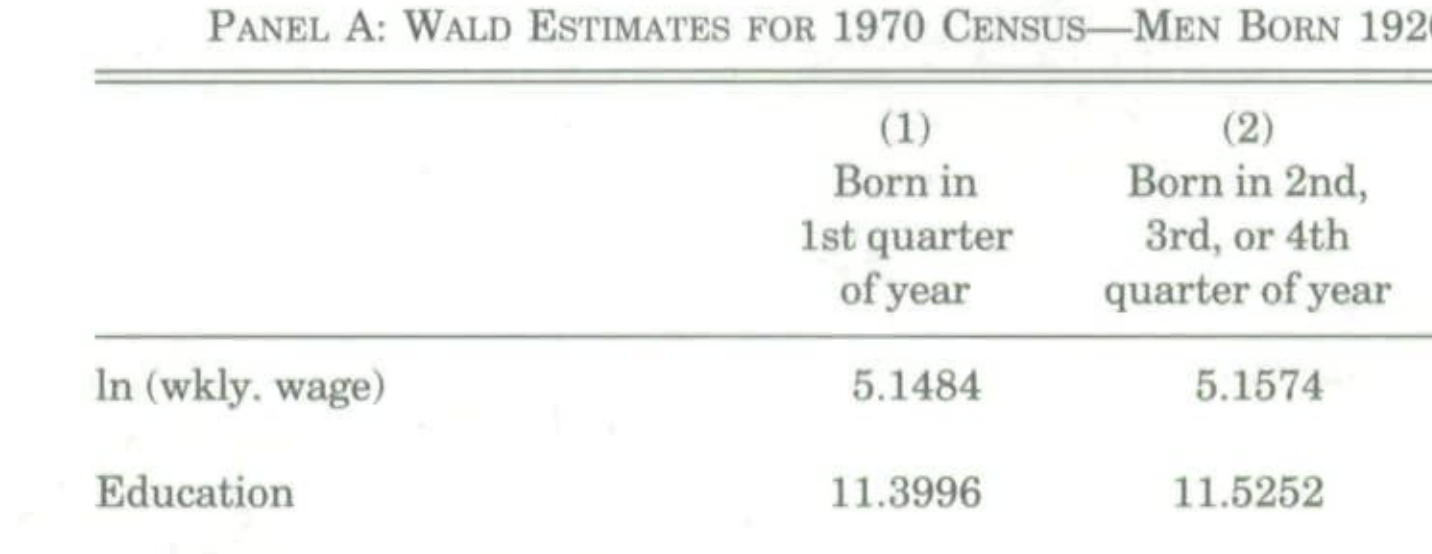
\includegraphics[width = 0.5\linewidth]{../Chapter7/ak-first-stage-basic}

	\begin{wideitemize}
		\item
		Under the four key assumptions, $\beta_{IV} = \frac{ E[Y_i | Z_i = 1] - E[Y_i | Z_i = 0] }{E[D_i | Z_i = 1] - E[D_i | Z_i = 0]}$ identifies a LATE (average treatment effect for compliers) 
		
		\item
		Estimation is done by plugging in sample analogs for reduced form and first-stage, then taking the ratio
		
		\pause
		\item
		Estimation 2: can also be done by ``two-stage least squares'', which allows us to incorporate multiple instruments (make sure you know how) 
			\begin{wideitemize}
				\item
				Regress $D_i$ on instrument $Z_i$ (and controls)
				
				\item
				Regress $Y_i$ on predictions $\hat{D}_i$ (and controls)
			\end{wideitemize}
	\end{wideitemize}
	
\end{frame}

\begin{frame}{RDD}
	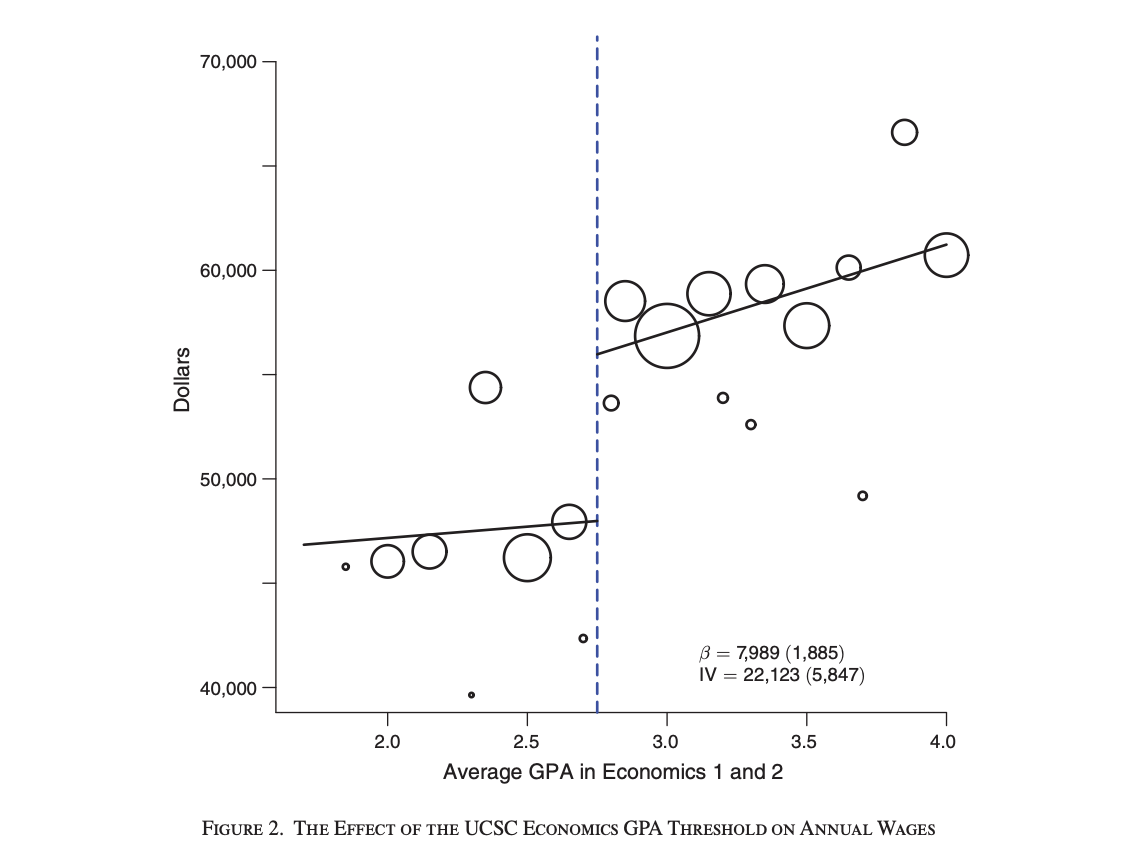
\includegraphics[width = 0.5 \linewidth]{../Chapter8/bleemer-rf}
	
	\begin{wideitemize}
		\item
		In RDD, we compare people just above/below a threshold that (partially) determines treatment status
		
		\pause
		\item
		Identification: potential outcomes are continuous at the cutoff
			\begin{itemize}
				\item 
				Make sure you understand when this might fail!
			\end{itemize}
		
		\pause
		\item
		Estimation: estimate CEF at the cutoff using OLS or local linear regression
			\begin{wideitemize}
				\item
				Note: I will not test you on the details of local linear regression
			\end{wideitemize}
	\end{wideitemize}
\end{frame}


\begin{frame}{Concluding thoughts I}
We've done a lot in one semester! \medskip

\begin{wideitemize}
	\item
	Learned about the challenges of estimating causal effects
	
	\item
	Developed statistical language to help us think about when/how we can learn about causal effects
	
	\item
	Learned several applicable ``identification strategies'' for learning about causal effects
	
	\item
	Developed tools for estimating and testing hypotheses about causal effects in finite samples (often using regression!)
\end{wideitemize}

\pause
\medskip
There's still a lot more to learn, if you're interested in taking more classes!
	\begin{itemize}
		\item 
		Non-parametrics, machine learning approaches, Bayesian econometrics, time series and forecasting, etc.
	\end{itemize}

\end{frame}

\begin{frame}{Concluding thoughts II}
There are many different ways that I hope you can apply these tools going forward: \medskip

\begin{wideitemize}
	\item
	Do research that helps to improve policies or firm decisions, thereby increasing social welfare (or corporate profits - your choice!)
	
		\begin{itemize}
			\item 
			If you're interested in academic research, I encourage you to work as a research assistant for profs at Brown and/or write an honors thesis
		\end{itemize}
	
	\item
	Better understand empirical evidence as you read articles in the newspaper, online, etc.
	
	\item
	Become an econometrician and help to develop tools for getter policy analysis in the future :-) 
	
	
\end{wideitemize}

	
\end{frame}


\begin{frame}{Concluding thoughts III}
	\begin{wideitemize}
		\item
		I encourage you to fill out the course evaluation/feedback form: \href{https://brown.evaluationkit.com  }{\underline{https://brown.evaluationkit.com}}
		
		\item
		Course feedback will be used both for evaluation purposes and for trying to improve the course!
		
		\item
		This is my third time teaching this course, so any comments on what worked or could have been done better are much appreaciated. Thanks!
	\end{wideitemize}
\end{frame}

\begin{frame}
	\centering
	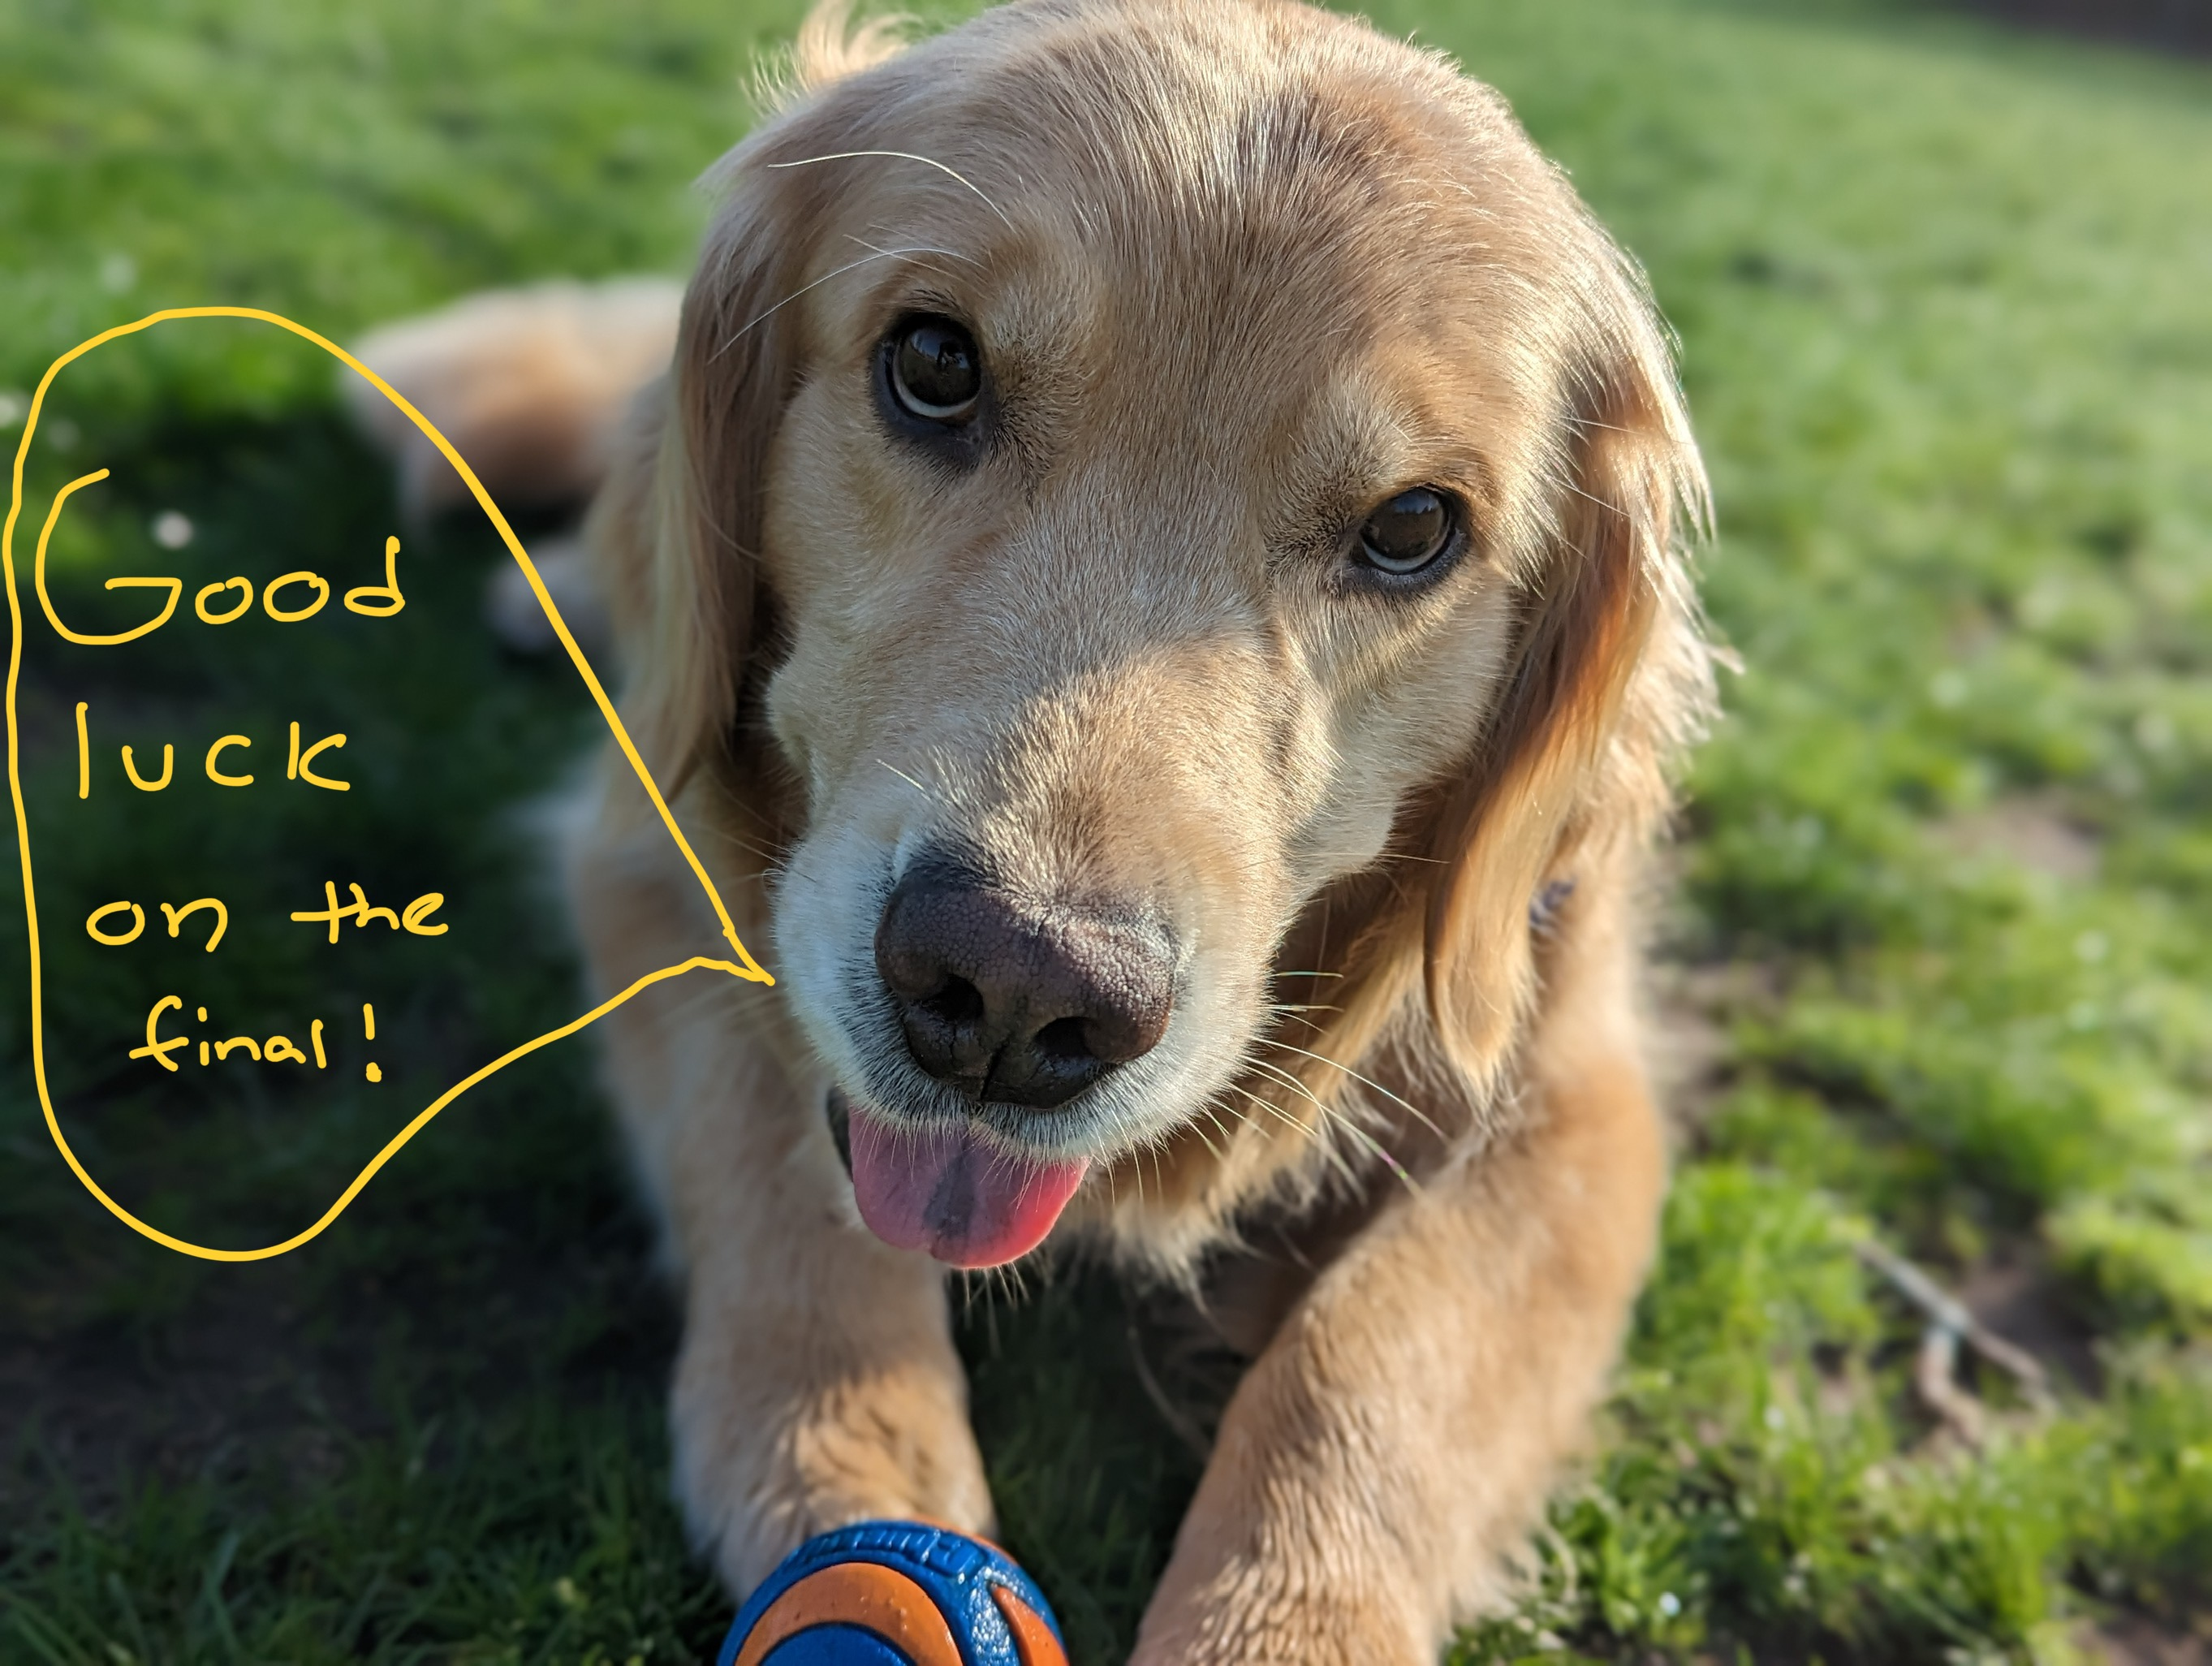
\includegraphics[width = 0.9 \linewidth]{poppy-good-luck}
\end{frame}

\end{document}


